\documentclass[]{book}
\usepackage{lmodern}
\usepackage{amssymb,amsmath}
\usepackage{ifxetex,ifluatex}
\usepackage{fixltx2e} % provides \textsubscript
\ifnum 0\ifxetex 1\fi\ifluatex 1\fi=0 % if pdftex
  \usepackage[T1]{fontenc}
  \usepackage[utf8]{inputenc}
\else % if luatex or xelatex
  \ifxetex
    \usepackage{mathspec}
  \else
    \usepackage{fontspec}
  \fi
  \defaultfontfeatures{Ligatures=TeX,Scale=MatchLowercase}
\fi
% use upquote if available, for straight quotes in verbatim environments
\IfFileExists{upquote.sty}{\usepackage{upquote}}{}
% use microtype if available
\IfFileExists{microtype.sty}{%
\usepackage{microtype}
\UseMicrotypeSet[protrusion]{basicmath} % disable protrusion for tt fonts
}{}
\usepackage[margin=1in]{geometry}
\usepackage{hyperref}
\hypersetup{unicode=true,
            pdftitle={From Novice to Expert In Bioinformatics},
            pdfauthor={Shaojun Xie},
            pdfborder={0 0 0},
            breaklinks=true}
\urlstyle{same}  % don't use monospace font for urls
\usepackage{natbib}
\bibliographystyle{apalike}
\usepackage{color}
\usepackage{fancyvrb}
\newcommand{\VerbBar}{|}
\newcommand{\VERB}{\Verb[commandchars=\\\{\}]}
\DefineVerbatimEnvironment{Highlighting}{Verbatim}{commandchars=\\\{\}}
% Add ',fontsize=\small' for more characters per line
\usepackage{framed}
\definecolor{shadecolor}{RGB}{248,248,248}
\newenvironment{Shaded}{\begin{snugshade}}{\end{snugshade}}
\newcommand{\KeywordTok}[1]{\textcolor[rgb]{0.13,0.29,0.53}{\textbf{{#1}}}}
\newcommand{\DataTypeTok}[1]{\textcolor[rgb]{0.13,0.29,0.53}{{#1}}}
\newcommand{\DecValTok}[1]{\textcolor[rgb]{0.00,0.00,0.81}{{#1}}}
\newcommand{\BaseNTok}[1]{\textcolor[rgb]{0.00,0.00,0.81}{{#1}}}
\newcommand{\FloatTok}[1]{\textcolor[rgb]{0.00,0.00,0.81}{{#1}}}
\newcommand{\ConstantTok}[1]{\textcolor[rgb]{0.00,0.00,0.00}{{#1}}}
\newcommand{\CharTok}[1]{\textcolor[rgb]{0.31,0.60,0.02}{{#1}}}
\newcommand{\SpecialCharTok}[1]{\textcolor[rgb]{0.00,0.00,0.00}{{#1}}}
\newcommand{\StringTok}[1]{\textcolor[rgb]{0.31,0.60,0.02}{{#1}}}
\newcommand{\VerbatimStringTok}[1]{\textcolor[rgb]{0.31,0.60,0.02}{{#1}}}
\newcommand{\SpecialStringTok}[1]{\textcolor[rgb]{0.31,0.60,0.02}{{#1}}}
\newcommand{\ImportTok}[1]{{#1}}
\newcommand{\CommentTok}[1]{\textcolor[rgb]{0.56,0.35,0.01}{\textit{{#1}}}}
\newcommand{\DocumentationTok}[1]{\textcolor[rgb]{0.56,0.35,0.01}{\textbf{\textit{{#1}}}}}
\newcommand{\AnnotationTok}[1]{\textcolor[rgb]{0.56,0.35,0.01}{\textbf{\textit{{#1}}}}}
\newcommand{\CommentVarTok}[1]{\textcolor[rgb]{0.56,0.35,0.01}{\textbf{\textit{{#1}}}}}
\newcommand{\OtherTok}[1]{\textcolor[rgb]{0.56,0.35,0.01}{{#1}}}
\newcommand{\FunctionTok}[1]{\textcolor[rgb]{0.00,0.00,0.00}{{#1}}}
\newcommand{\VariableTok}[1]{\textcolor[rgb]{0.00,0.00,0.00}{{#1}}}
\newcommand{\ControlFlowTok}[1]{\textcolor[rgb]{0.13,0.29,0.53}{\textbf{{#1}}}}
\newcommand{\OperatorTok}[1]{\textcolor[rgb]{0.81,0.36,0.00}{\textbf{{#1}}}}
\newcommand{\BuiltInTok}[1]{{#1}}
\newcommand{\ExtensionTok}[1]{{#1}}
\newcommand{\PreprocessorTok}[1]{\textcolor[rgb]{0.56,0.35,0.01}{\textit{{#1}}}}
\newcommand{\AttributeTok}[1]{\textcolor[rgb]{0.77,0.63,0.00}{{#1}}}
\newcommand{\RegionMarkerTok}[1]{{#1}}
\newcommand{\InformationTok}[1]{\textcolor[rgb]{0.56,0.35,0.01}{\textbf{\textit{{#1}}}}}
\newcommand{\WarningTok}[1]{\textcolor[rgb]{0.56,0.35,0.01}{\textbf{\textit{{#1}}}}}
\newcommand{\AlertTok}[1]{\textcolor[rgb]{0.94,0.16,0.16}{{#1}}}
\newcommand{\ErrorTok}[1]{\textcolor[rgb]{0.64,0.00,0.00}{\textbf{{#1}}}}
\newcommand{\NormalTok}[1]{{#1}}
\usepackage{longtable,booktabs}
\usepackage{graphicx,grffile}
\makeatletter
\def\maxwidth{\ifdim\Gin@nat@width>\linewidth\linewidth\else\Gin@nat@width\fi}
\def\maxheight{\ifdim\Gin@nat@height>\textheight\textheight\else\Gin@nat@height\fi}
\makeatother
% Scale images if necessary, so that they will not overflow the page
% margins by default, and it is still possible to overwrite the defaults
% using explicit options in \includegraphics[width, height, ...]{}
\setkeys{Gin}{width=\maxwidth,height=\maxheight,keepaspectratio}
\IfFileExists{parskip.sty}{%
\usepackage{parskip}
}{% else
\setlength{\parindent}{0pt}
\setlength{\parskip}{6pt plus 2pt minus 1pt}
}
\setlength{\emergencystretch}{3em}  % prevent overfull lines
\providecommand{\tightlist}{%
  \setlength{\itemsep}{0pt}\setlength{\parskip}{0pt}}
\setcounter{secnumdepth}{5}
% Redefines (sub)paragraphs to behave more like sections
\ifx\paragraph\undefined\else
\let\oldparagraph\paragraph
\renewcommand{\paragraph}[1]{\oldparagraph{#1}\mbox{}}
\fi
\ifx\subparagraph\undefined\else
\let\oldsubparagraph\subparagraph
\renewcommand{\subparagraph}[1]{\oldsubparagraph{#1}\mbox{}}
\fi

%%% Use protect on footnotes to avoid problems with footnotes in titles
\let\rmarkdownfootnote\footnote%
\def\footnote{\protect\rmarkdownfootnote}

%%% Change title format to be more compact
\usepackage{titling}

% Create subtitle command for use in maketitle
\newcommand{\subtitle}[1]{
  \posttitle{
    \begin{center}\large#1\end{center}
    }
}

\setlength{\droptitle}{-2em}
  \title{From Novice to Expert In Bioinformatics}
  \pretitle{\vspace{\droptitle}\centering\huge}
  \posttitle{\par}
\subtitle{Linux, Perl and R for Bioinformatics}
  \author{Shaojun Xie}
  \preauthor{\centering\large\emph}
  \postauthor{\par}
  \predate{\centering\large\emph}
  \postdate{\par}
  \date{2016-12-23}

\usepackage{booktabs}

\usepackage{xcolor}

\lstset{
    basicstyle=\ttfamily,
    numbers=left,
    numberstyle=\footnotesize,
    stepnumber=2,
    numbersep=5pt,
    backgroundcolor=\color{black!10},
    showspaces=false,
    showstringspaces=false,
    showtabs=false,
    tabsize=2,
    captionpos=b,
    breaklines=true,
    breakatwhitespace=true,
    breakautoindent=true,
    linewidth=\textwidth
}

\begin{document}
\maketitle

{
\setcounter{tocdepth}{1}
\tableofcontents
}
\chapter{Preface}\label{preface}

\section{About me}\label{about-me}

I'm a husband, a father, a son, a brother and a researcher. My name is
Shaojun Xie. I started to work on analyzing next generation sequencing
(NGS) data in 2010. When I first heard of NGS, I was an undergraduate
student at Huazhong Agricultural University in China. When I began to do
my PhD in China Agricultural University (CAU), more and more researchers
around me started to talk about NGS data. At that time, I had no idea
about what NGS was. In the first year of my PhD (2009), my wet
experiment was not smooth. I thought I need to make some change. I think
bioinformatics is a cool area. Then I checked online for job
advertisements related to bioinformatics to see what the employers need.
I figured out that Linux, Perl and R were the most important things
needed. After that I started to read the book (Perl: How to program).
Also I started to use Ubuntu which a variant of Linux. I can understood
the contents in the book. But I didn't know what I should do or what I
can do with the knowledge I learned from the book.

A few months later (September in 2010), I joined a new lab and started
to analyze RNA-seq data. The results of that work was later published in
PNAS. I'm one of the co-first authors. Although I was responsible for
parts of the project, it helped me a lot. I learned how to use Perl and
R in the data analysis. That project opened the door for me. After that
I worked on several other projects. Meanwhile, we had several
collaborations with other labs. These different projects broadened my
horizon in the area of NGS data analysis. Some of the projects were
published in high profile journals, like Genome Research, Plant Cell,
etc.

In June 2014, I graduated from China Agricultural University. One of my
collaborators recommended me to another lab. I got a position as a
research associate. This position also provided me an opportunity to be
a visiting scholar at Purdue University. I got Purdue University in
August 2014. I worked on several nice projects. Some of them also got
published in nice journals. One year later, I started to look for a job
as a bioinformatician. Bioinformatics Core was just recruiting
bioinformaticians at that time. I got an offer and then joined the core
in April 2014. Currently I'm a bioinformatician in Bioinformatics Core
at Purdue University.

\section{ Who should read this book?}\label{who-should-read-this-book}

I started to do NGS data analysis as a bench researcher. I started from
ZERO. I understand how people feel when they were ZERO. So this book is
written for researchers who have no prior knowledge of NGS data
analysis. You do NOT need any programming background. If you already
have some, that's good. All you need is the strength and the resolution
to finish this book.

For those of you who already have some experience but you still don't
feel comfortable when dealing with the data, this will be for you. In
this book, I will write some skills that I have learned, which will
accelerate your analysis.

\chapter{First Perl Program}\label{first-perl-program}

As all other programming books, we begin with a ``Hello world'' program.

\begin{Shaded}
\begin{Highlighting}[]
\KeywordTok{#!/usr/bin/perl}
\CommentTok{#Printing a line of text “Hello, Bioinformatics”}
\FunctionTok{print} \KeywordTok{"}\StringTok{Hello, Bioinformatics!}\CharTok{\textbackslash{}n}\KeywordTok{"}\NormalTok{;}
\end{Highlighting}
\end{Shaded}

This program show how to display a line a text in Perl. It have several
features. We go through each line in detail. Line 1 is what we call
shebang line. This line starts with shebang construct (\texttt{\#!}).
\texttt{/usr/bin/perl} indicates the path of the Perl interpreter.

Line 3 shows how to print a line of text in Perl. Nearly all programming
language use print to display texts on the screen. Here, print is a
built-in function in Perl. It print the string of characters (its
arguments) between quotation marks (``'' or `').

\begin{Shaded}
\begin{Highlighting}[]
\KeywordTok{perl} \NormalTok{code_perl/hello_bioinfor.pl}
\end{Highlighting}
\end{Shaded}

\begin{verbatim}
Hello, Bioinformatics!
\end{verbatim}

\begin{Shaded}
\begin{Highlighting}[]
\KeywordTok{ls} \NormalTok{-l code_perl/hello_bioinfor.pl}
\KeywordTok{code_perl/hello_bioinfor.pl}
\end{Highlighting}
\end{Shaded}

\begin{verbatim}
-rwxr-xr-x 1 Shaojun 197609 106 Dec 21 14:56 code_perl/hello_bioinfor.pl
Hello, Bioinformatics!
\end{verbatim}

\begin{Shaded}
\begin{Highlighting}[]
\KeywordTok{chmod} \NormalTok{755 code_perl/hello_bioinfor.pl}
\KeywordTok{perl} \NormalTok{code_perl/hello_bioinfor.pl}
\end{Highlighting}
\end{Shaded}

\begin{verbatim}
Hello, Bioinformatics!
\end{verbatim}

\begin{Shaded}
\begin{Highlighting}[]
\CommentTok{## Remove execute permission }
\KeywordTok{chmod} \NormalTok{600 code_perl/hello_bioinfor.pl}
\KeywordTok{ls} \NormalTok{-l code_perl/hello_bioinfor.pl}
\end{Highlighting}
\end{Shaded}

\begin{verbatim}
-rwxr-xr-x 1 Shaojun 197609 106 Dec 21 14:56 code_perl/hello_bioinfor.pl
\end{verbatim}

After we press ENTER on the keyboard, the program will execute and
display the output in Figure 5.1 if the program is syntactically
correct. However the characters \texttt{\textbackslash{}n} are not
displayed. Here backslash \texttt{\textbackslash{}} is a start of an
escape sequence. It changes the meaning of the character after it. The
backslash \texttt{\textbackslash{}} and \texttt{n} together
(\texttt{\textbackslash{}n}) form an escape sequence and signify a
newline. Other examples are \texttt{\textbackslash{}t} (tab) or
\texttt{\textbackslash{}\$} (= print an actual dollar sign, normally a
dollar sign has a special meaning). We'll see more escape sequences in
7.1. You can try to remove \texttt{\textbackslash{}n} in the program to
see what will happen. This will give you a more understanding of the
program.

\section{Varible}\label{varible}

In order to tell the computer what to print, we need to use variables.
In Perl, the name of a variable starts with the dollar sign \texttt{\$}.
You can assign either a number or a string to it.

\begin{Shaded}
\begin{Highlighting}[]
\KeywordTok{#!/usr/bin/perl -w}
\FunctionTok{use} \KeywordTok{strict}\NormalTok{;}

\CommentTok{#assign 2 numbers to 2 variable}

\KeywordTok{my} \DataTypeTok{$dna1} \NormalTok{= }\KeywordTok{"}\StringTok{CTCGACCAGGACGATGAATGGGCGATGAAAATCT}\KeywordTok{"}\NormalTok{;}
\KeywordTok{my} \DataTypeTok{$dna2} \NormalTok{= }\KeywordTok{"}\StringTok{CGCTAAACGCTAAACCCTAAACGCTAAACCTCTGAATCCTTAATCGCT}\KeywordTok{"}\NormalTok{;}

\CommentTok{#Returns the length in characters of the value of EXPR}
\KeywordTok{my} \DataTypeTok{$dna_length1} \NormalTok{= }\FunctionTok{length} \DataTypeTok{$dna1}\NormalTok{; }
\KeywordTok{my} \DataTypeTok{$dna_length2} \NormalTok{= }\FunctionTok{length} \DataTypeTok{$dna2}\NormalTok{;}

\FunctionTok{print} \KeywordTok{"}\StringTok{First DNA: }\KeywordTok{"}\NormalTok{, }\DataTypeTok{$dna1}\NormalTok{, }\KeywordTok{"}\CharTok{\textbackslash{}n}\KeywordTok{"}\NormalTok{;}
\FunctionTok{print} \KeywordTok{"}\StringTok{Second DNA: }\KeywordTok{"}\NormalTok{, }\DataTypeTok{$dna1}\NormalTok{, }\KeywordTok{"}\CharTok{\textbackslash{}n}\KeywordTok{"}\NormalTok{;}

\CommentTok{#calculate the total length of two DNA sequences}
\KeywordTok{my} \DataTypeTok{$tot_length} \NormalTok{= }\DataTypeTok{$dna_length1} \NormalTok{+ }\DataTypeTok{$dna_length2}\NormalTok{;}
\FunctionTok{print} \KeywordTok{"}\StringTok{The total length of two DNA sequences is }\DataTypeTok{$tot_length}\StringTok{ }\CharTok{\textbackslash{}n}\KeywordTok{"}\NormalTok{;}

\CommentTok{# calculate the average length of two DNA sequences. }
\KeywordTok{my} \DataTypeTok{$average_length} \NormalTok{= (}\DataTypeTok{$dna_length1} \NormalTok{+ }\DataTypeTok{$dna_length2}\NormalTok{) / }\DecValTok{2}\NormalTok{;}
\FunctionTok{print} \KeywordTok{"}\StringTok{The average length of two DNA sequences is }\DataTypeTok{$average_length}\StringTok{ }\CharTok{\textbackslash{}n}\KeywordTok{"}\NormalTok{;}

\CommentTok{#calulate the differences between the two DNA sequences}
\KeywordTok{my} \DataTypeTok{$diff_length} \NormalTok{= }\DataTypeTok{$dna_length2} \NormalTok{- }\DataTypeTok{$dna_length1}\NormalTok{;}
\FunctionTok{print} \KeywordTok{"}\StringTok{The length difference of two DNA sequences is }\KeywordTok{"}\NormalTok{, }\DataTypeTok{$diff_length}\NormalTok{, }\KeywordTok{"}\CharTok{\textbackslash{}n}\KeywordTok{"}\NormalTok{;}

\CommentTok{#Imaging the CC content of first DNA sequence is 0.5. }
\CommentTok{#How many CC do we have in first DNA?}
\KeywordTok{my} \DataTypeTok{$cg_content} \NormalTok{= }\FloatTok{0.5}\NormalTok{;}
\KeywordTok{my} \DataTypeTok{$cg_number} \NormalTok{= }\DataTypeTok{$dna_length1} \KeywordTok{*} \FloatTok{0.5}\NormalTok{;}

\CommentTok{#Imaging we have a 10 bps DNA sequnces, }
\CommentTok{#how many possible DNA sequences do we have?}
\KeywordTok{my} \DataTypeTok{$dna_nucleotide} \NormalTok{= }\KeywordTok{"}\StringTok{ATCG}\KeywordTok{"}\NormalTok{;}
\KeywordTok{my} \DataTypeTok{$dna_nucleo_number} \NormalTok{= }\FunctionTok{length} \DataTypeTok{$dna_nucleotide}\NormalTok{;}
\KeywordTok{my} \DataTypeTok{$dna_length} \NormalTok{= }\DecValTok{10}\NormalTok{;}
\KeywordTok{my} \DataTypeTok{$possible_number} \NormalTok{= }\DataTypeTok{$dna_nucleo_number} \NormalTok{*}\KeywordTok{*} \DataTypeTok{$dna_length}\NormalTok{;}
\FunctionTok{print} \KeywordTok{"}\StringTok{We have }\DataTypeTok{$possible_number}\StringTok{ possibilities.}\CharTok{\textbackslash{}n}\KeywordTok{"}\NormalTok{;}
\end{Highlighting}
\end{Shaded}

\chapter{Introduction}\label{intro}

You can label chapter and section titles using \texttt{\{\#label\}}
after them, e.g., we can reference Chapter \ref{intro}. If you do not
manually label them, there will be automatic labels anyway, e.g.,
Chapter \ref{methods}.

Figures and tables with captions will be placed in \texttt{figure} and
\texttt{table} environments, respectively.

\begin{Shaded}
\begin{Highlighting}[]
\KeywordTok{par}\NormalTok{(}\DataTypeTok{mar =} \KeywordTok{c}\NormalTok{(}\DecValTok{4}\NormalTok{, }\DecValTok{4}\NormalTok{, .}\DecValTok{1}\NormalTok{, .}\DecValTok{1}\NormalTok{))}
\KeywordTok{plot}\NormalTok{(pressure, }\DataTypeTok{type =} \StringTok{'b'}\NormalTok{, }\DataTypeTok{pch =} \DecValTok{19}\NormalTok{)}
\end{Highlighting}
\end{Shaded}

\begin{figure}

{\centering \includegraphics[width=0.8\linewidth]{bookdown-demo_files/figure-latex/nice-fig-1} 

}

\caption{Here is a nice figure!}\label{fig:nice-fig}
\end{figure}

Reference a figure by its code chunk label with the \texttt{fig:}
prefix, e.g., see Figure \ref{fig:nice-fig}. Similarly, you can
reference tables generated from \texttt{knitr::kable()}, e.g., see Table
\ref{tab:nice-tab}.

\begin{Shaded}
\begin{Highlighting}[]
\NormalTok{knitr::}\KeywordTok{kable}\NormalTok{(}
  \KeywordTok{head}\NormalTok{(iris, }\DecValTok{20}\NormalTok{), }\DataTypeTok{caption =} \StringTok{'Here is a nice table!'}\NormalTok{,}
  \DataTypeTok{booktabs =} \OtherTok{TRUE}
\NormalTok{)}
\end{Highlighting}
\end{Shaded}

\begin{table}

\caption{\label{tab:nice-tab}Here is a nice table!}
\centering
\begin{tabular}[t]{rrrrl}
\toprule
Sepal.Length & Sepal.Width & Petal.Length & Petal.Width & Species\\
\midrule
5.1 & 3.5 & 1.4 & 0.2 & setosa\\
4.9 & 3.0 & 1.4 & 0.2 & setosa\\
4.7 & 3.2 & 1.3 & 0.2 & setosa\\
4.6 & 3.1 & 1.5 & 0.2 & setosa\\
5.0 & 3.6 & 1.4 & 0.2 & setosa\\
\addlinespace
5.4 & 3.9 & 1.7 & 0.4 & setosa\\
4.6 & 3.4 & 1.4 & 0.3 & setosa\\
5.0 & 3.4 & 1.5 & 0.2 & setosa\\
4.4 & 2.9 & 1.4 & 0.2 & setosa\\
4.9 & 3.1 & 1.5 & 0.1 & setosa\\
\addlinespace
5.4 & 3.7 & 1.5 & 0.2 & setosa\\
4.8 & 3.4 & 1.6 & 0.2 & setosa\\
4.8 & 3.0 & 1.4 & 0.1 & setosa\\
4.3 & 3.0 & 1.1 & 0.1 & setosa\\
5.8 & 4.0 & 1.2 & 0.2 & setosa\\
\addlinespace
5.7 & 4.4 & 1.5 & 0.4 & setosa\\
5.4 & 3.9 & 1.3 & 0.4 & setosa\\
5.1 & 3.5 & 1.4 & 0.3 & setosa\\
5.7 & 3.8 & 1.7 & 0.3 & setosa\\
5.1 & 3.8 & 1.5 & 0.3 & setosa\\
\bottomrule
\end{tabular}
\end{table}

You can write citations, too. For example, we are using the
\textbf{bookdown} package \citep{R-bookdown} in this sample book, which
was built on top of R Markdown and \textbf{knitr} \citep{xie2015}.

\chapter{Why Linux?}\label{why-linux}

\section{What is Linux}\label{what-is-linux}

Before the creation of Linux, Unix was developed by AT\&T Bell Labs in
the 1960's. It's an operating system. Before the creation of Linux, and
before the rise of Windows, the computing world was dominated by Unix
(from web). After many years of evolution, Linux was created in early
1990's.

In case you don't know, Mac OS X is also a certified Unix operating
system. So most of the Linux skills are applied in Mac OS X.

Linux is a clone of the operating system Unix, written from scratch by
Linus Torvalds (Figure \ref{fig:LinuxTerminal}) with assistance from a
loosely-knit team of hackers across the Net. It aims towards POSIX and
Single UNIX Specification compliance (Torvalds, 2015).



\begin{Shaded}
\begin{Highlighting}[]
\NormalTok{knitr::}\KeywordTok{include_graphics}\NormalTok{(}\StringTok{"figures/linux_terminal_example.png"}\NormalTok{)}
\end{Highlighting}
\end{Shaded}

\begin{figure}
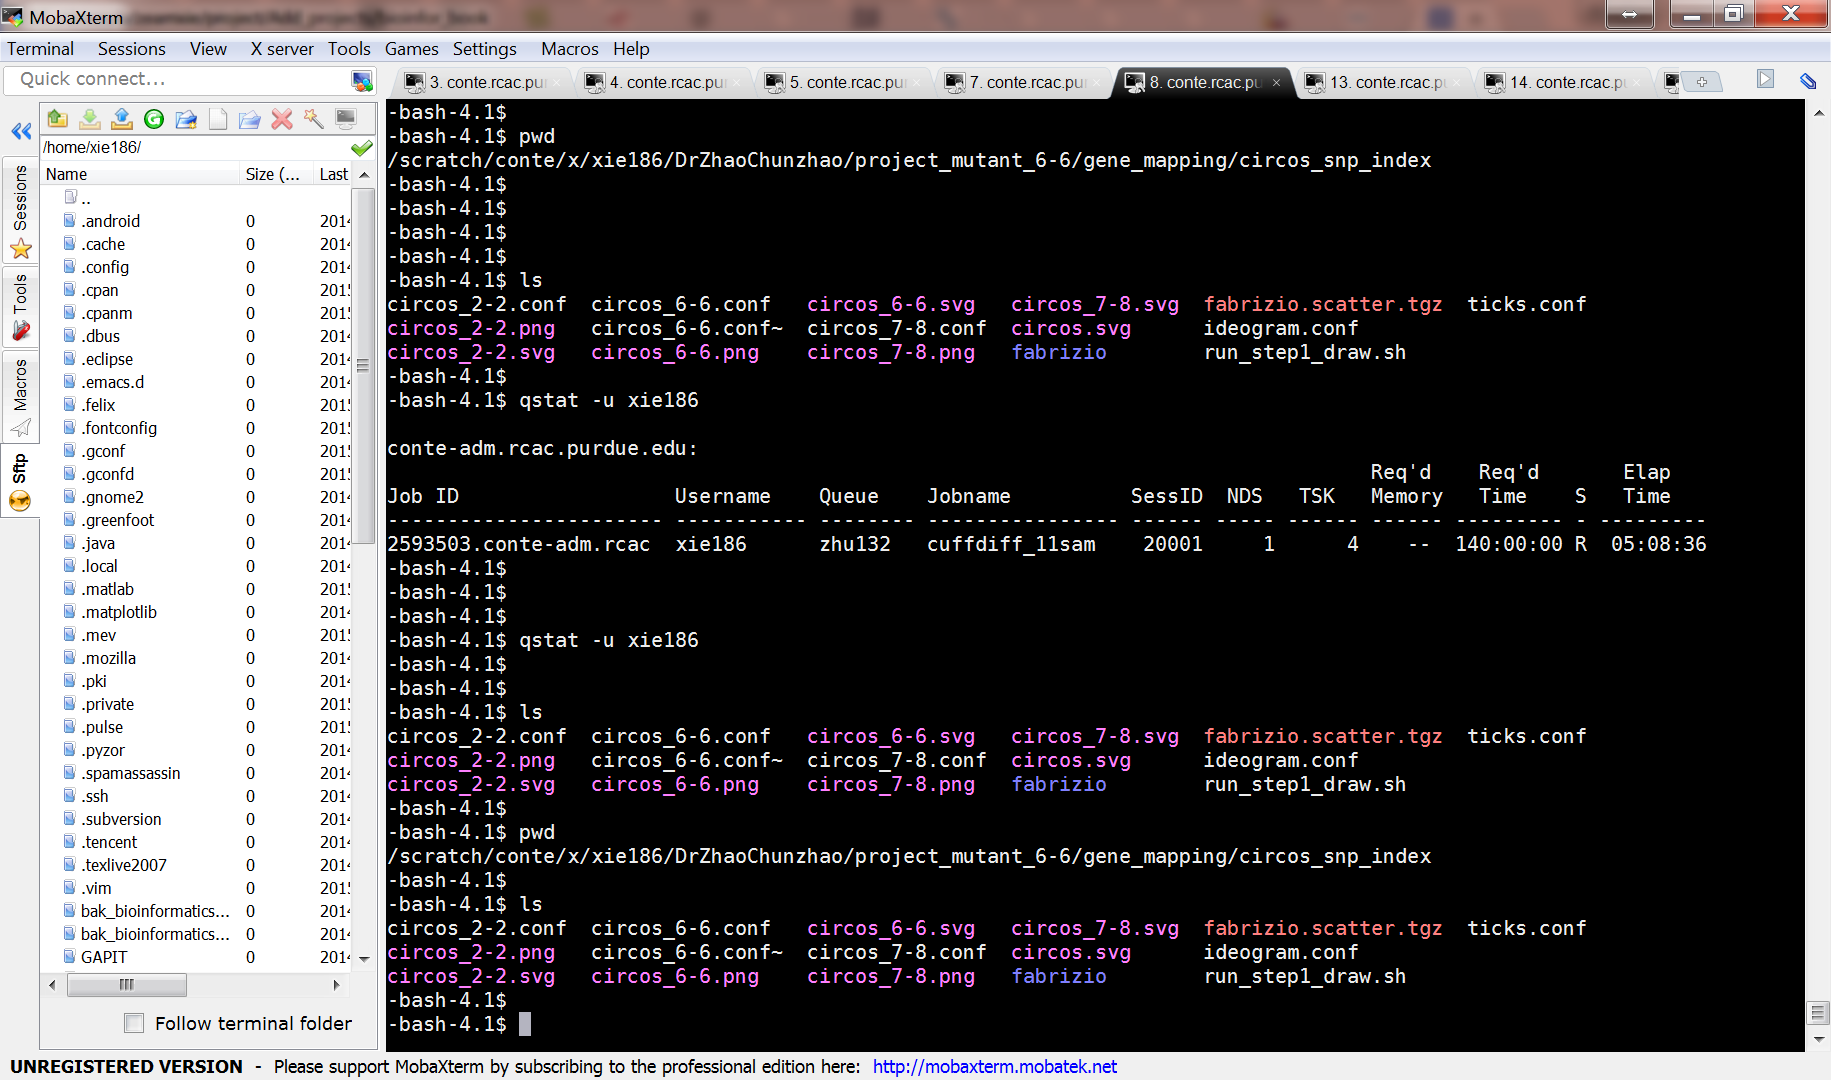
\includegraphics[width=1\linewidth]{figures/linux_terminal_example} \caption{An example of Linux terminal.}\label{fig:LinuxTerminal}
\end{figure}

\chapter{Literature}\label{literature}

Here is a review of existing methods.

\chapter{Methods}\label{methods}

We describe our methods in this chapter.

\chapter{Applications}\label{applications}

Some \emph{significant} applications are demonstrated in this chapter.

\section{Example one}\label{example-one}

\section{Example two}\label{example-two}

\chapter{Final Words}\label{final-words}

We have finished a nice book.

\chapter{Practical Perl program}\label{practical-perl-program}

\section{Extracting sequences from genomic DNA for some specific
regions}\label{extracting-sequences-from-genomic-dna-for-some-specific-regions}

Figure 8.1 shows how to extract sequences from genomic DNA for some
specific regions. For example, when we perform ChIP-seq for a
transcription factor. We will get the binding sites (some regions) of
transcription factor after analyzing ChIP-seq. You want to know whether
there is motifs that can be recognized by the transcription factor.

The Perl program in Figure 8.1 has two arguments (input files): genomic
DNA sequences and ChIP-seq peak regions. It will print the genomic DNA
sequences for each region in fasta format. We can use
\texttt{\textgreater{}} to generate a new file to record the result
(Figure 8.1).

The genomic DNA sequence data is saved in fasta format (See 11.1).
ChIP-seq peak regions are saved in BED format (See 12.3).

Let's go through each line in detail.

A normal paragraph.

The above code provides an interactive HTML page (figure \ref{fig:foo})




\begin{Shaded}
\begin{Highlighting}[]
\KeywordTok{plot}\NormalTok{(}\DecValTok{1}\NormalTok{)  }\CommentTok{# a scatterplot}
\end{Highlighting}
\end{Shaded}

\begin{figure}[htbp]
\centering
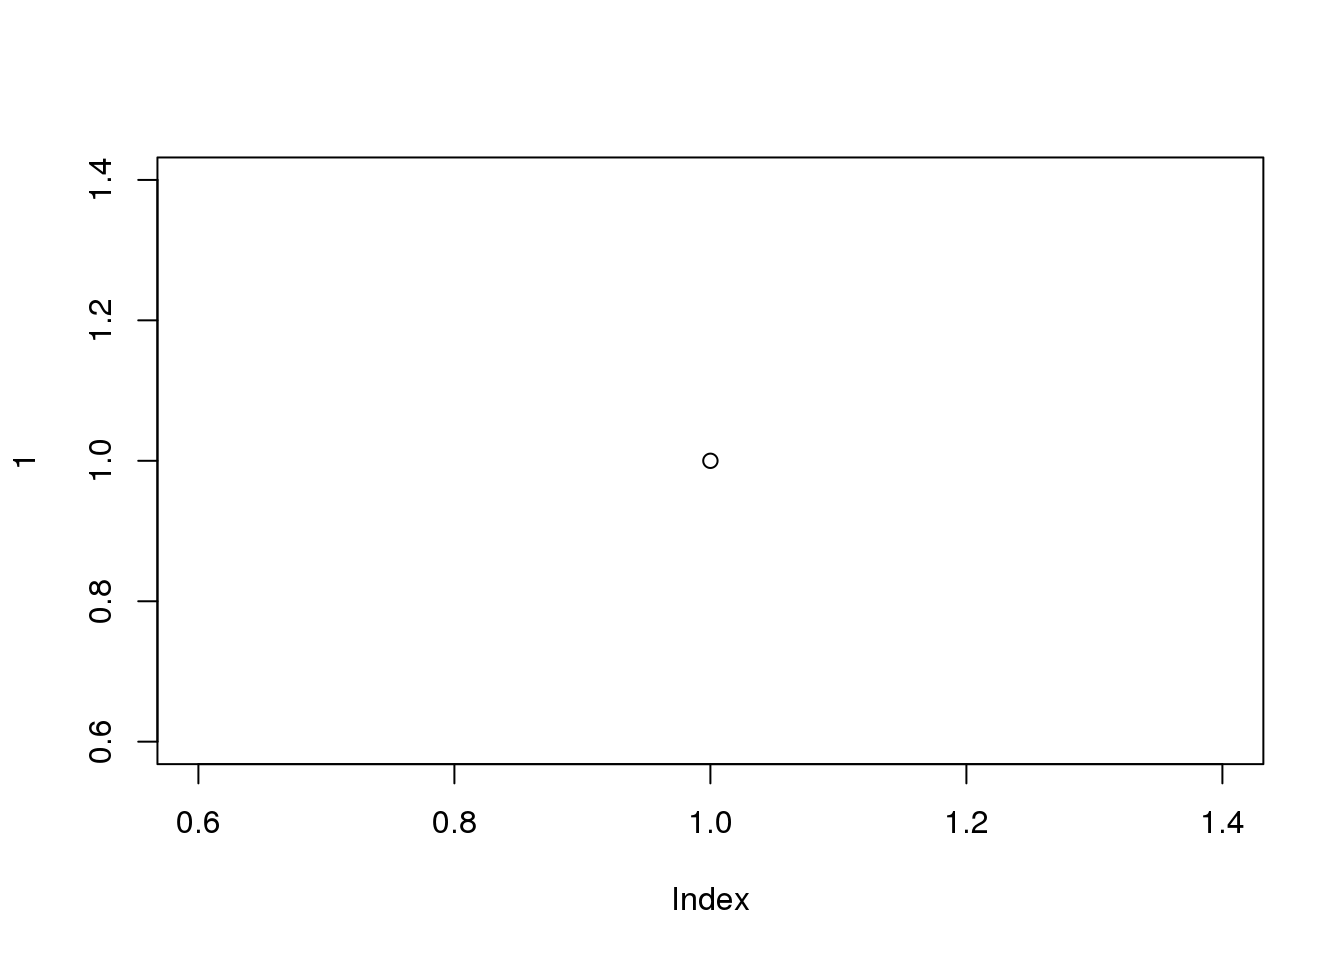
\includegraphics{bookdown-demo_files/figure-latex/foo-1.pdf}
\caption{\label{fig:foo}A scatterplot of the data \texttt{cars} using \textbf{base} R
graphics.}
\end{figure}

\bibliography{packages,book}


\end{document}
